\section{Microcontroller validation}
\label{sec:str7_validation_microcontroller_validation}

The previous sections focused on the validation of the ARM7TDMI processor simulator at user and system level.
In this section, the target of the validation is the complete microcontroller under study\footnote{We would like to thank Schneider Electric, and specially Khaled Rahmouny for his collaboration on the validation of the UNISIM STR7 microcontroller simulator. Without their collaboration, the validation of the simulator on an industrial environment could not have been possible. For confidentiality issues the applications used during the validation and modules added on the simulator are not discussed in this document.} (see Figure~\ref{fig:str7_validation_str7_architecture}).
In order to validate the microcontroller a full application that boots the device and uses the different peripherals was necessary, and preferably a real world application.
For that purpose Schneider Electric has provided the software necessary to run the microcontroller and extended the simulator desing with an external DSP and a graphical interface of the Schneider Electric product embedding the STR7 microcontroller.

\begin{figure}[!h]
	\begin{center}
		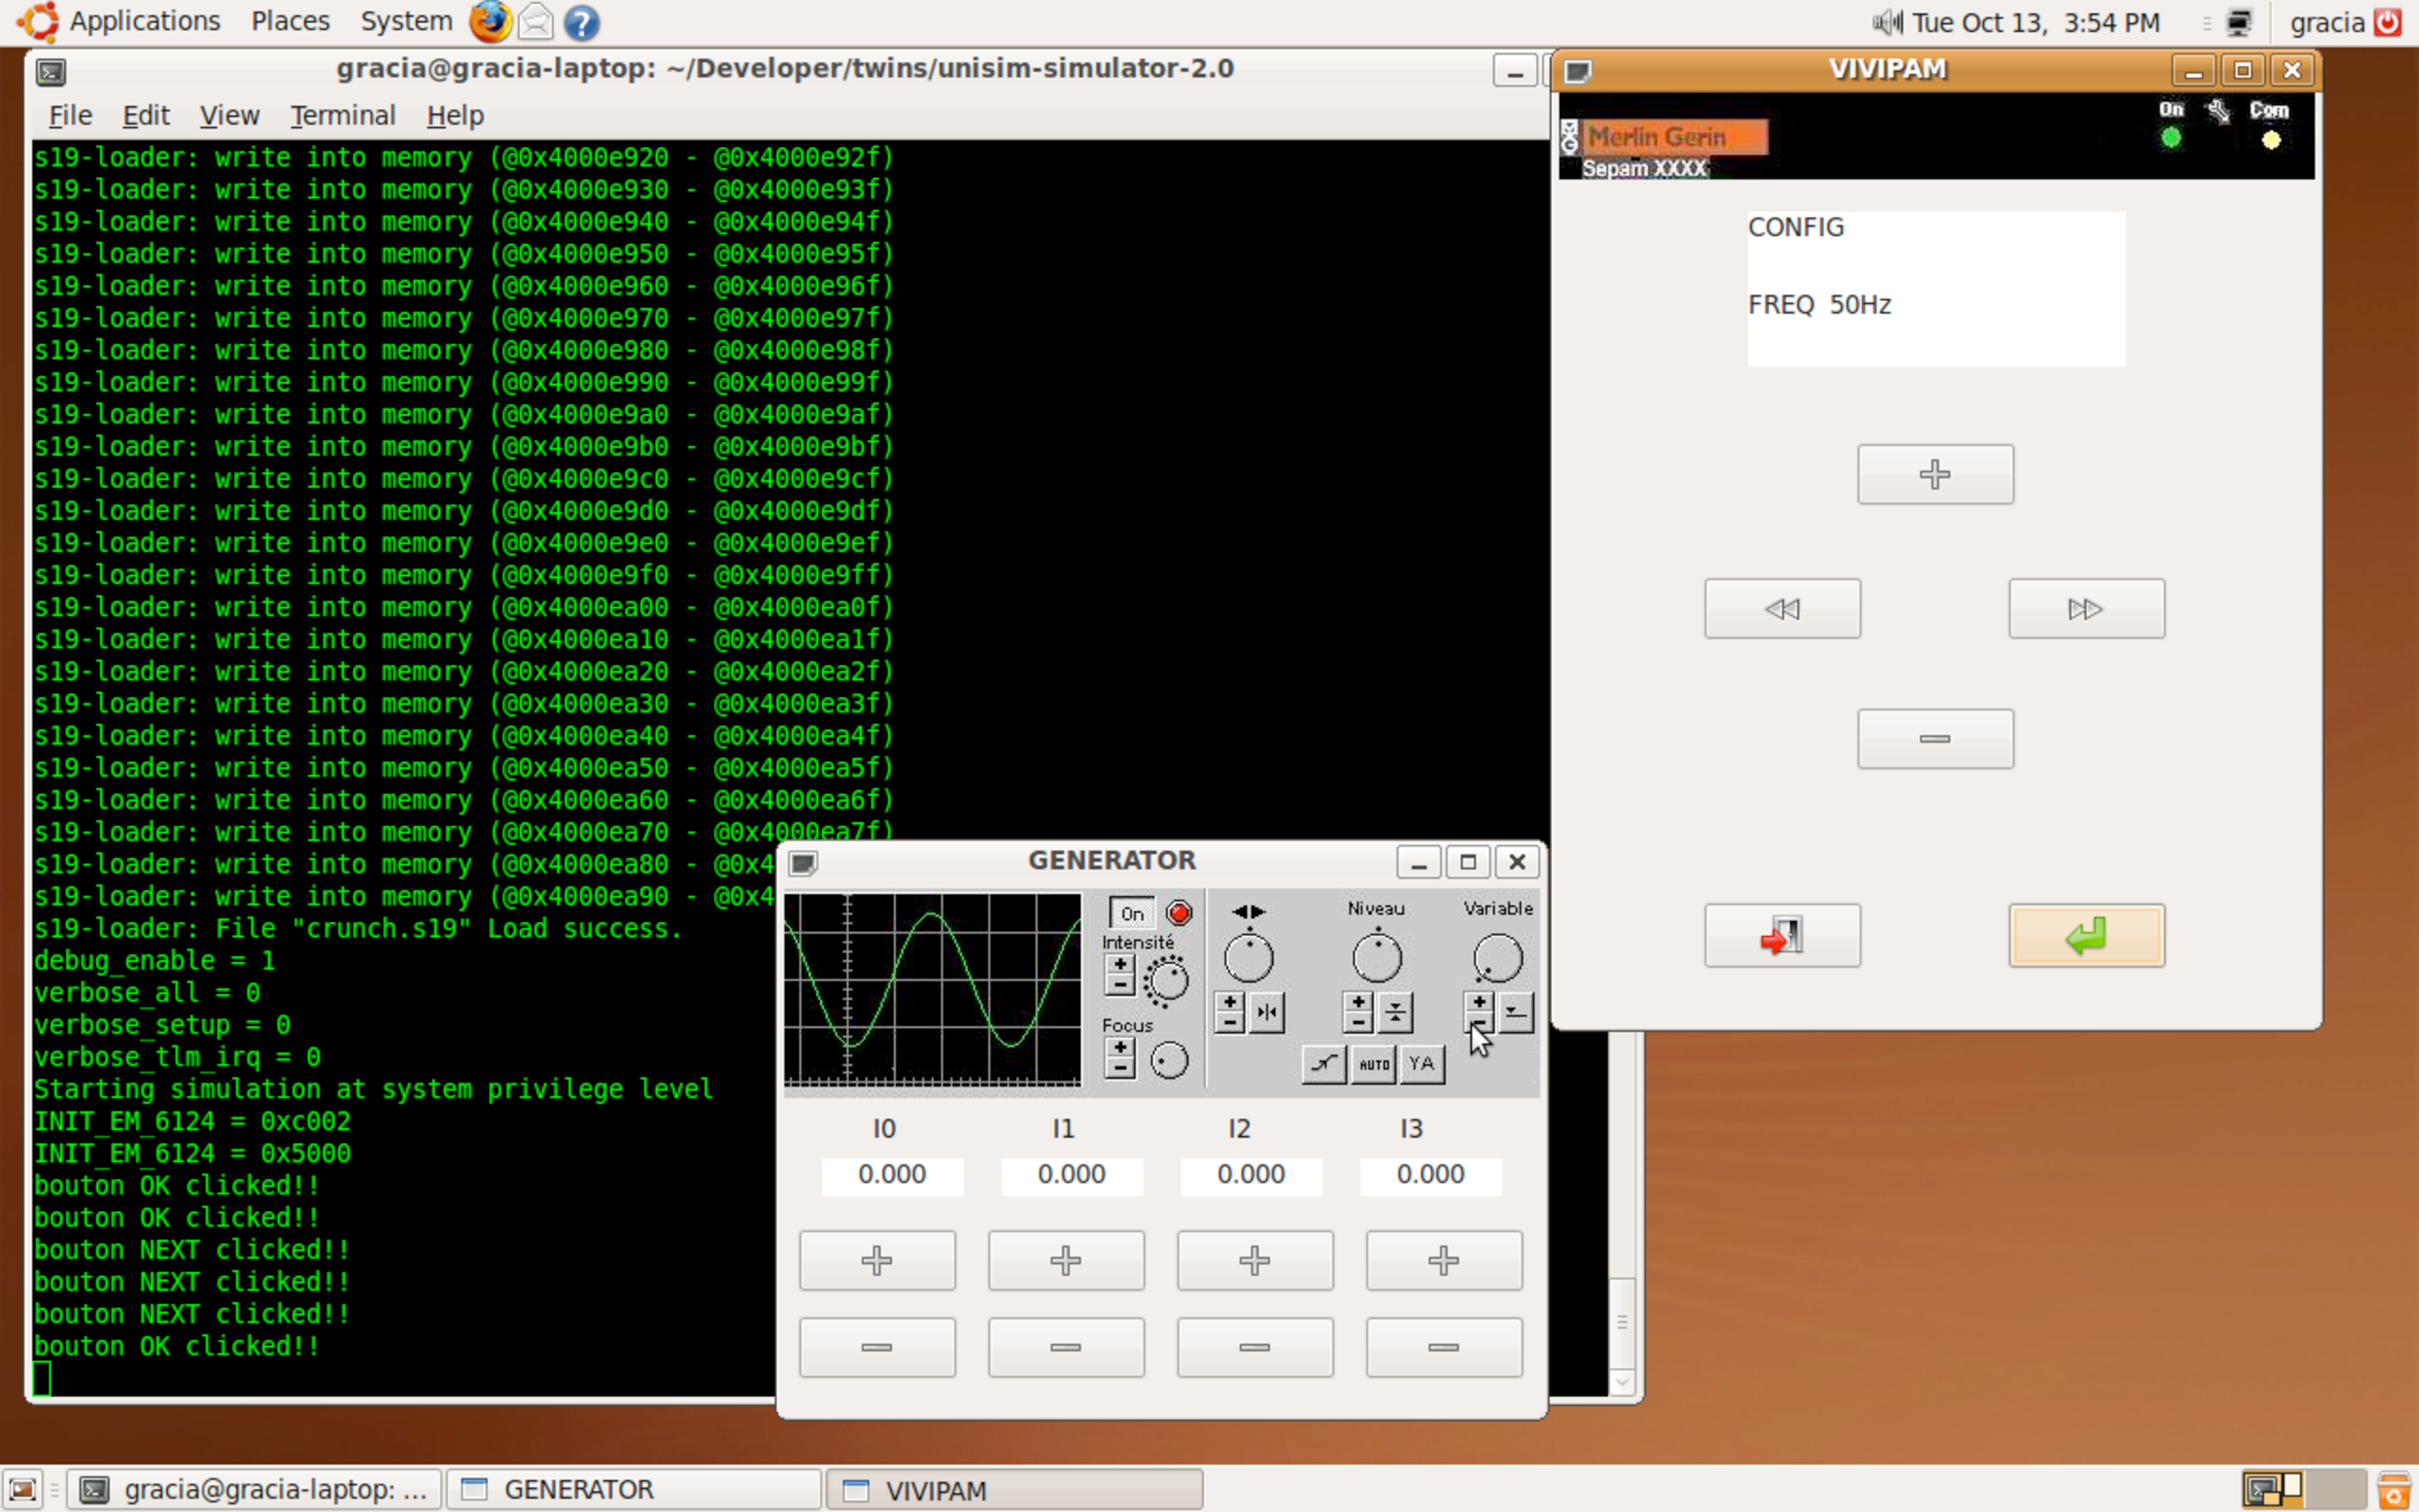
\includegraphics[width=\textwidth]{str7_validation/figures/industrial.pdf}
	\end{center}
	\caption{Industrial application running on top of the STR7 simulator.}
	\label{fig:str7_validation_industrial_application}
\end{figure}

The validation of the microcontroller has been done progressively and all the capabilities of the simulator were tested.
The steps followed during the validation were:
\begin{enumerate}
	\item ELF and S19 loaders test.
	\item Microprocessor boot process validation.
	\item Validation of bus communications, mainly with the RAM and the FLASH memories.
	\item Procesor validation using a regression test software used by Schneider Electric.
	\item Validation of the interruption handling, this includes the both the processor and the interrupt controller.
	\item Timers capabilities validation.
	\item Validation of the BSPI communication peripheral. For this test the BSPI peripheral was connected to the external DSP developed by Schneider Electric.
	\item Validation of the GPIO peripherals.
	\item Validation of the complete system using a industrial application.
\end{enumerate}
For each of the validation steps a STR7 software provided by Schneider Electric was used, which was augmented as each step validation was successfully passed.
Figure~\ref{fig:str7_validation_industrial_application} shows the final program running on top of the simulator.

The functional behavior of the simulator of the microcontroller simulator was validated against a real system using the same STR7 microcontroller.
Additionally timing tests were run to check the time precision of the simulator.

\subsection{Results}

The functional behavior of the different components of the simulator and of the simulator as a whole has been validated, thanks to the use of the industrial application.

The timing behavior currently differs with the real platform. 
Our tests showed that the simulated software is slightly slower than on the real platform.
However, the slightly different timings do not impact on the development of industrial applications over the simulator.

